%%mark = star, diamond, square, otimes
%\documentclass{article}
%\usepackage{pgfplots}
%\usepackage[justification=centering]{caption}
%\pgfplotsset{compat=newest}
%\begin{document}
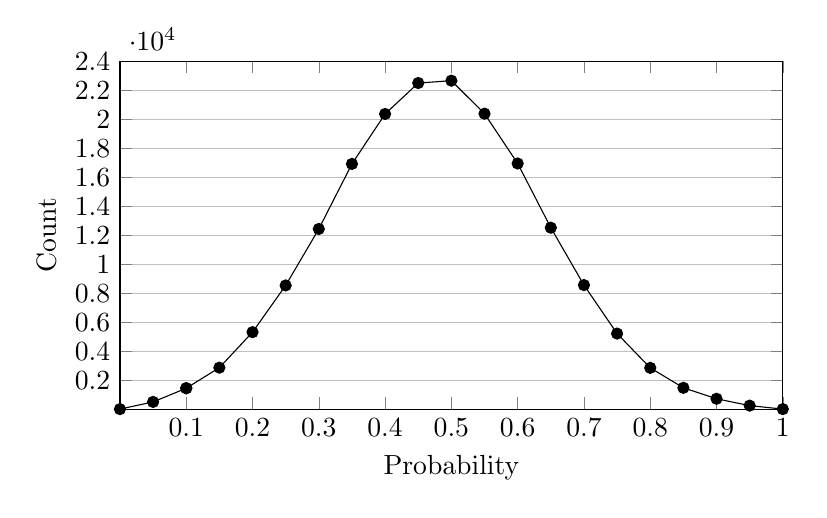
\begin{tikzpicture}
\begin{axis}[
 width=10cm,
   height=6cm,
    xlabel={Probability },
    ylabel={Count},
    xmin=0, xmax=1.0,
    ymin=0, ymax=24000,
    xtick={.1,.2,.3,.4,.5,.6,.7,.8,.9,1.0},
    ytick={2000,4000,6000,8000,10000,12000,14000,16000,18000,20000,22000,24000},
    legend pos=north east,
    ymajorgrids=true,
    grid style={line width=.2pt,draw=gray!50},
]
 
\addplot[
    solid, every mark/.append style={solid, fill=black}, mark=*
    ]
    coordinates {
		(0,0)
		(.05,495)
		(0.1,1439)
		(0.1 ,1439)
		(0.15,2859)
		(0.2 ,5307)
		(0.25,8531)
		(0.3 ,12426)
		(0.35,16915)
		(0.4 ,20358)
		(0.45,22493)
		(0.5 ,22655)
		(0.55,20380)
		(0.6 ,16943)
		(0.65,12514)
		(0.7 ,8555)
		(0.75,5209)
		(0.8 ,2845)
		(0.85,1468)
		(0.9 ,712)
		(0.95,240)
		(1.0,0)
};
 
\end{axis}
\end{tikzpicture}
%\end{document}